\documentclass{article}
\usepackage[utf8]{inputenc}
\usepackage{fancyhdr}
\usepackage{graphicx}
\usepackage{hyperref}
\usepackage{geometry}


% ---- Commands ------- %
\newcommand{\documentNumber}[1]{
    \LARGE  \textbf{ PUSS2142{#1} } \\
    \medskip
}
\newcommand{\documentVersion}[1]{
    v. {#1}

    \medskip
}
\newcommand{\documentTitle}[1]{
    \centerline{\rule{13cm}{0.4pt}}
    \bigskip \bigskip
    \LARGE {#1} \\
    \bigskip \bigskip
    \centerline{\rule{13cm}{0.4pt}}
}
\newcommand{\documentGroup}[1]{
    \bigskip \bigskip
    \LARGE Group {#1} \\
    \bigskip
}
\newcommand{\documentResponsible}[1]{
    \LARGE Responsible: {#1} \\
    \medskip
}
\newcommand{\documentAuthors}[1]{
    \LARGE Authors: {#1} \\
    \medskip    
}
\newcommand{\documentDate}[1]{
    \date {#1} 
}

\graphicspath{{./images/}} % Defines a path to file images
\renewcommand{\arraystretch}{1.7}  % Vertical padding for tables

% --- Header & Footer ---- %
\pagestyle{fancy}
\lhead{\leftmark}
\rhead{}
\rfoot{\thepage}
\cfoot{}
\lfoot{}


% ------------------------------------------------ #


\title {
    \documentNumber {00}    % Must be 2 digits
    \documentVersion {1.0}
    \documentTitle {Software Development Plan}
    \documentGroup {2}
    \documentResponsible {Project Management Group}
    \documentAuthors {Project Management Group}
    \documentDate {2021-02-12}
}

\begin{document}

\maketitle
\thispagestyle{empty}

\newpage

\tableofcontents

\newpage

\section{Document History}
\begin{tabular}{ l | l | l | l }
    Version & Date & Responsible & Description \\
    \hline
    0.1 & 2021-01-25 & PG & Document created. \\
    0.2 & 2021-02-02 & PG & Ready for informal review. \\
    0.3 & 2021-02-04 & PG & Corrected grammatical changes and typos. \\
    0.4 & 2021-02-10 & PG & Corrected typos and clarified the usage of E-PUSS. \\
    0.5 & 2021-02-10 & PG & Corrected typos after second informal review. \\
    1.0 & 2021-02-12 & PG & Reached baseline. \\
\end{tabular}

\section{Introduction}
    This document describes the development model and the development plan for TimeMate.
    TimeMate is a system for time reporting and is based on \textit{Baseblock System} and will be developed by students at LTH for the course
    \textit{ETSF20 Programvaruutveckling för stora projekt}.

\section{Terminology}
    
    See table \ref{Terminology}.
    
    \begin{table}[h]
        \centering
        \begin{tabular}{| l | l |}
            \hline
                SG & System management Group \\
            \hline
                DG & Developer Group \\
            \hline
                TG & Test Group \\
            \hline
                PG & Project Management Group \\
            \hline 
                CML & Configuration item Management List \\
            \hline            
                ECG & Error Control Group \\
            \hline
                SDP & Software Development Plan \\
            \hline
                SRS & Software Requirements Specification \\
            \hline
                SVVS & Software Verification and Validation Specification \\
            \hline
                SVVI & Software Verification and Validation Instruction \\
            \hline
                STLDD & Software Top Level Design Document \\
            \hline
                SDDD & Software Detailed Design Document \\
            \hline
                SVVR & Software Verification and Validation Report \\
            \hline
                SSD & System Specification Document \\
            \hline
                PFR & Project Final Report \\
            \hline
                IRP & Informal Review Protocol \\
            \hline
        \end{tabular}
        \caption{Terminology}
        \label{Terminology}
    \end{table}

\section{Referenced Documents \label{refs}}
    \begin{itemize}
        \item Software Requirements Specification: BaseBlockSystem, v. 1.0, Doc. number: PUSS12002
        \item \href{https://docs.oracle.com/javase/specs/jls/se11/html/index.html}{The Java Language Specification, Java SE 11 Edition}.
        \item \label{PH} Project Instruction (Projekthandledningen).
        \item Informal Review Protocol, v. 0.1, Doc. number: PUSS214210.
        \item Configuration item Management List, v. 0.1, Doc. number: PUSS214209.
    \end{itemize}
    

\section{Development Model} %Assar och Victor
    The development model in this project is the waterfall model. This
    means that the project is divided into four seperate phases where each phase depends
    on the previous one in a sequential manner. It is thus required that a phase is
    completed before the next one begins.
    \\ \\
    In every phase, several documents must be produced (see table \ref{documenttable}) and a phase
    is considered completed only once all documents required in the phase have reached baseline.
    To reach baseline, all documents of the phase must first pass an informal review, 
    followed by a formal review. This process and its details is further described in section \ref{followup}.
    
\section{Staff Organisation} %Assar
    The group consists of 21 members divided into 4 main groups, with 2 extra groups consisting of members from several groups. 
    
    \subsection{Project Management Group}
        \textbf{Members: (2)}
        \begin{itemize}
            \item Assar Orpana
            \item Victor Krook
        \end{itemize}
        \textbf{Responsibilities:}
        \begin{itemize}
            \item Coordinating the group effort.
            \item Creating a project plan and making sure that it is followed.
            \item Ensuring that every individual has the information they need.
            \item Authoring the following documents.
                \begin{itemize}
                    \item SDP
                    \item SSD
                    \item PFR
                \end{itemize} 
        \end{itemize}
        
    \subsection{Software Architecture Group}
        \textbf{Members: (4)}
        \begin{itemize}
            \item David Vilppu
            \item Ramtin Mosavi
            \item Filip Sjövall
            \item Mustafa Elomeiri
        \end{itemize}
        \textbf{Responsibilities}
        \begin{itemize}
            \item Designing the software architecture.
            \item Delegating work to DG and TG.
            \item Coordinating and co-authoring of the following documents.
                \begin{itemize}
                    \item SRS
                    \item STLDD
                    \item SDDD
                    \item PFR
                \end{itemize} 
        \end{itemize}
 
    \subsection{Development Group}
        \textbf{Members: (10)}
        \begin{itemize}
            \item Alexandra Galonja
            \item Anna Bergvall
            \item Annelie Sinander
            \item Hjalmar Janson
            \item Oscar Johansson
            \item Sebastian Forslund
            \item Abd Salam
            \item Alaa Wahbah
            \item Alexander Olofsson
            \item Johan Wulf
        \end{itemize}
        \textbf{Responsibilities}
        \begin{itemize}
            \item Designing the UI for the software.
            \item Developing the architecture designed by SG.
            \item Developing the code for the system.
            \item Co-authoring the following documents.
                \begin{itemize}
                    \item SRS
                    \item STLDD
                    \item STDDD
                    \item PFR
                \end{itemize}
        \end{itemize}
    
    \subsection{Test Group}
        \textbf{Members: (5)}
        \begin{itemize}
            \item Alexander Möhle
            \item Lazar Trpeski
            \item Max Palmgren
            \item Malte Wallander
            \item Anas Abu Al-Soud
        \end{itemize}
        \textbf{Responsibilities}
        \begin{itemize}
            \item Testing and validating the functionality of code written by DG.
            \item Authoring the following documents.
            \begin{itemize}
                \item SVVS
                \item SVVI
            \end{itemize}
            \item Co-authoring the following documents.
                \begin{itemize}
                    \item SRS
                    \item PFR
                \end{itemize}
        \end{itemize}
    
    \subsection{Group Leaders}
        \textbf{Members: (3)}
        \begin{itemize}
            \item Oscar Johansson (DG)
            \item Alexander Möhle (TG)
            \item David Vilppu (SG)
        \end{itemize}
        \textbf{Responsibilities: }
        \begin{itemize}
            \item Coordinating work efforts between the groups. 
            \item Reporting progress to PG.
            \item Organizing work shifts for their respective groups. 
        \end{itemize}
        
    \subsection{Error control group}
        \textbf{Members: (7)}
        \begin{itemize}
            \item Assar Orpana (PG)
            \item Victor Krook (PG)
            \item David Vilppu (SG)
            \item Ramtin Mosavi (SG)
            \item Filip Sjövall (SG)
            \item Mustafa Elomeiri (SG)
        \end{itemize}
        \textbf{Responsibilities: }
        \begin{itemize}
            \item Managing error reports.
            \item Handling Configuration management.
            \item Updating baseline documents.  
        \end{itemize}

    \subsection{Others}
        The forementioned groups make up the team responsible for developing the software. Other stakeholders include:
        \begin{itemize}
            \item \textbf{Head of section:} Oversees the project and has direct contact with the client. 
            \item \textbf{Client:} Provides a requirement specification.
            \item \textbf{Experts:} Provides auxiliary knowledge in their respective fields.
            \item \textbf{Examiner:} Performs the formal review.
        \end{itemize}

\section{Schedule}
    The project starts in week 3 and ends in week 12, which means there are 9 weeks available. In every phase, several documents shall be produced and table \ref{documenttable} illustrates which documents should be produced for each phase. Figure \ref{schedule} illustrates the estimated time for each phase and the estimated days scheduled for meetings, informal reviews and formal reviews (see section \ref{informalreview}).
    \begin{table}[h]
        \centering
        \begin{tabular}{| c | p{0.2\textwidth} |}
            \hline
                \textbf{Phase} & \textbf{Document} \\
            \hline
                1 &   \begin{minipage}[t]{0.4\textwidth}
                        \begin{itemize}
                            \item SRS
                            \item SVVS
                            \item SDP \\
                        \end{itemize} 
                        \end{minipage} \\
             \hline
                2 &
                \begin{minipage}[t]{0.4\textwidth}
                \begin{itemize}
                        \item SVVI
                        \item STLDD \\
                    \end{itemize}
                    \end{minipage} \\
             \hline
                3 & 
                \begin{minipage}[t]{0.4\textwidth}
                \begin{itemize}
                        \item SDDD \\
                    \end{itemize}
                    \end{minipage} \\
             \hline
                4 & 
                \begin{minipage}[t]{0.4\textwidth}
                \begin{itemize}
                        \item SVVR
                        \item SSD
                        \item PFR \\
                    \end{itemize}
                    \end{minipage} \\
             \hline
        \end{tabular}
        \caption{Documents to be produced for each phase}
        \label{documenttable}
    \end{table}
    
    \begin{figure}[h]
        \centering
        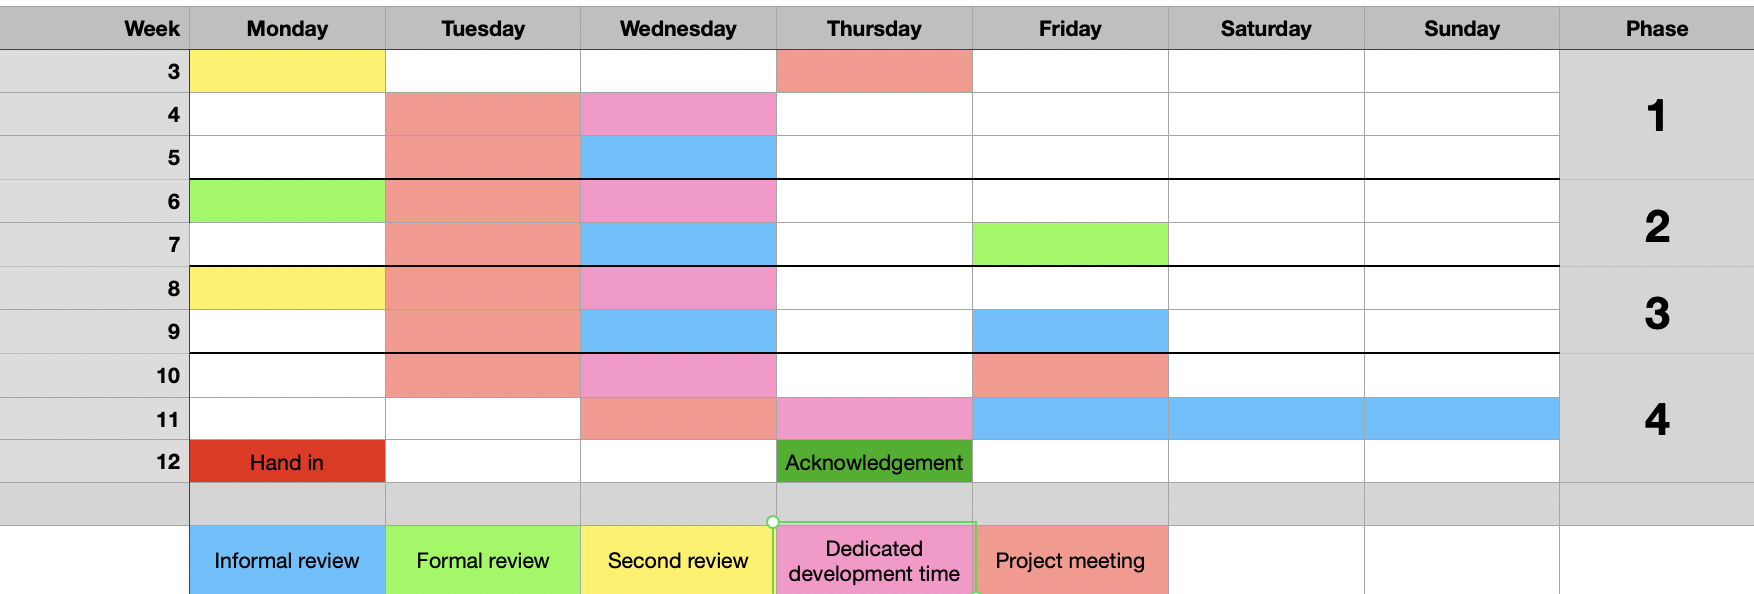
\includegraphics[width=\textwidth]{images/schedule.png}
        \caption{Estimated project schedule}
        \label{schedule}
    \end{figure}
    
    \subsection{Project Group Meetings \label{PM}}
        Project Group Meetings will be held on Tuesdays and these meetings will be mandatory for each member in the group.
        These meetings will be used to discuss the project and take general decisions. This is an important step in the development model, to ensure that everyone is on the same page and that the time plan is being kept.

    \subsection{Estimated Work Load}
        PG holds a one hour long meeting every week and has scheduled for a two hour time slot every Wednesday during which every group works on their respective task. To supplement this, the groups are expected to manage their own planning meetings and work sessions. Since the workload of each group varies between phases, it seems more fitting to allow groups the flexibility of managing their own time. Group leaders are tasked with making sure that coordination between groups is constant throughout the project. PG also estimates that approximately an hour every week will be spent on general discussions in the discord channel.
        \\ \\
        Table \ref{phasetable} illustrates the estimated start and end dates 
        for every phase, as well as estimated hours spent per week, per person.
        \begin{table}[h]
            \centering
            \begin{tabular}{|c|c|c|c|c|}
                \hline
                    \textbf{Phase} & \textbf{Start} & \textbf{End} & \textbf{Work days} & 
                    \textbf{Estimated hours/week} \\
                \hline
                    1 & 18/1 & 5/2 & 15 & 10 \\
                 \hline
                    2 & 08/2 & 19/2 & 10 & 10 \\
                 \hline
                    3 & 22/2 & 5/3  & 10 & 10 \\
                 \hline
                    4 & 8/3 & 19/3  & 10 & 15 \\
                 \hline
            \end{tabular}
            \caption{Estimated start dates and end for dates the phases}
            \label{phasetable}
        \end{table}
        \\
        Table \ref{activitytable} illustrates the estimated time spent per
        activity as well as how often the activity is expected to occur.
        
        \begin{table}[h]
            \centering
            \begin{tabular}{|l|c|c|}
                \hline
                    \textbf{Activity} & \textbf{Frequency/week} & \textbf{Duration (h)} \\
                \hline
                    Project group meeting & 1 & 1 \\
                 \hline
                    Project group work & 1 & 2 \\
                 \hline
                    Subgroup work session & 2 & 2*2 \\
                 \hline
                    Self studies & 1  & 1 \\
                 \hline
                    Discussions & 1 & 1 \\
                 \hline
                    Reviews/Expert meetings & 1 & 1 \\
                 \hline
                    \textbf{Total hours} & & \textbf{10} \\
                 \hline
            \end{tabular}
            \caption{Estimated time for each activity per person, per week}
            \label{activitytable}
        \end{table}
    

\section{Standards \& Tools}    % Victor
    In order to make the development process as easy and straight forward as possible,
    the project group has agreed on several standards and tools to use. 
    \\ \\
    The standards should be followed by every group member and consists of the following:
    \begin{itemize}
        \item The source code should follow Oracles ``The Java Language Specification".
        \item All comments, commits and pull-requests should be in english.
    \end{itemize}
    
    \subsection{Discord}
    Discord is used as the main communcation tool in the group. A server will be set up and is
    used for messaging as well as working together and having project meetings.
    The server consists of several voice channels and several text channels, each
    with its specific purpose, eg \textit{Meetings} or \textit{Developer Group}.
    
    \subsection{Github \& Git}
    Git is used for collaboration between documents and the project library (see \ref{project_library})
    and is hosted on Github. Git provides abilities that make certain actions very
    easy, such as pushing and pulling updates to the working repository and creating pull-requests for merging.
    
    \subsection{Eclipse}
        Eclipse is the primary IDE that is used due to it's huge span of functionality and the groups familiarity to it.
    
    \subsubsection{Egit}
        Egit is a plugin for Eclipse provides the tools needed for a git workflow 
        in Eclipse IDE.
        
    \subsubsection{Texmaker}
        Texmaker is a latex editor providing the tools needed to compile and preview latex files.
    
\section{Follow up and Quality Evaluation \label{followup}}
    To keep the quality of all documents as high as possible during the project,
    two reviews will be carried out at the end of every phase. One \textit{informal review}
    followed by one \textit{formal review}.

    \subsection{Informal Review \label{informalreview}}
        An informal review is performed within the project group and is meant to catch
        errors, bugs and mistakes in the documents. This is to ensure as high quality
        as possible for the formal review. The result of the review is \emph{not} pass or
        not pass, but its purpose is rather to improve the documents.
        \\ \\
        An informal review is carried out at least 3 days before the following formal review and the documents
        should be ready no later than 17:00 the day before the review. PG is responsible
        for coordinating the meetings as well as documenting them.
        There are at least three reviewers assigned for each document to be reviewed, and these
        are assigned by PG. During the review, the reviewers will mention and discuss what they have
        found and then the reviewees will get an opportunity to reply and have a discussion
        if needed. For a detailed description of how informal reviews are structured see IRP.
        \\ \\
        To emphasize, the informal review is \emph{not} ment to criticize or judge, but rather
        to make the documents as good as possible. 
        
    
    \subsection{Formal Review \label{formalreview}}
        After the documents have gone through the informal review, they must pass the formal review
        to reach baseline. During the formal review, an external reviewer is
        given the documents at least 48 hours in advance so that he or she can prepare.
        During the review, the entire project group shall be present.
        The formal review can result in one of the following scenarios:
        \begin{enumerate}
            \item The documents are approved.
            \item The documents are approved after certain modification.
            \item Modifications must be made followed by a re-review.
            \item The documents are \emph{not} approved and must be re-written,
                    followed by a new review.
        \end{enumerate}
    
    \subsection{Re-Review}
        In case the documents fail the formal review, it might be necessary to
        to do a new review after certain modifications have been made.
            
    \subsection{Following the Timeplan}
        If the project is unable to follow timeplan for some reason, the following steps should be taken:
        \begin{enumerate}
            \item \textbf{Identify the problem}: This is the most critical step of the            procedure because the cause could be anything from a bad timeplan to
                    members of the team being sick and unable to work.
            \item \textbf{Explore possible solutions}: Depending on what kind of problem has occured, there might be several different solutions and therefore it is important to identify and weigh the different ones.
            \item \textbf{Pick a solution}. 
            \item \textbf{Take an action}. 
            \item \textbf{Prevent the problem from happening again}:
                    To prevent the problem from happening again, there must be some
                    type of follow-up routine. Depending on what the problem scenario is,
                    this follow-up could be a personal meeting between PG and the persons
                    involved, or re-creating a timeplan using a different technique.
        \end{enumerate}

\section{Configuration Management}   % Victor
    All changes to items in the CML must follow a certain procedure once the documents
    have reached baseline. Git and Github are the main tools used for version control in this project.

    \subsection{Project Library \label{project_library}}
        The project library consists of two seperate libraries: Document libray and Work library.
    
        \subsubsection{Document Library \label{doclibrary}} %10.1.1
            The document library consists of the following:
            
            \begin{itemize}
                \item All configuration items that have reached baselines.
                \item Protocols from informal reviews (see section \ref{informalreview}).
                \item Protocols from formal reviews (see section \ref{formalreview}).
                \item Protocols and agendas from Project Group Meetings (see section \ref{PM}).
            \end{itemize}
            \noindent
            The purpose of this library is that the customer or a reviewer at any point should be able to access the forementioned. 
            This means that this library is initially almost empty, and documents are added as the project proceeds. In the end of phase 4, all items listed in CML can be found in this library.

        \subsubsection{Work Library}
            The work library contains all the files that are required during the project.
            The library is divided into three different branches where each branch has its unique purpose.
            
            \begin{itemize}
                \item \begin{verbatim} development \end{verbatim}
                This branch is where the all development is done and it is used as a placement for all files related
                to the project, regardless of their status.
                Every member in the group has free push access to this branch.
                
                \item \begin{verbatim} review \end{verbatim}
                Once the documents in the development branch are ready for an informal review,  they are moved
                into the \textit{review} branch. This requires a pull-request to be made, which must be reviewed and accepted by ECG before it is merged into the branch. 
                
                \item \begin{verbatim} master \end{verbatim}
                Once the documents pass the formal reviews, they are merged into 
                \textit{master} branch, which consists only of files that have reached baseline.
                Once new documents are added to this branch, they are also placed in the document library (see section \ref{doclibrary}).
                Note that not all files are copied to the document library, but only the documents specified in the CML.
            \end{itemize}
            
            \begin{figure}[h]
                \centering
                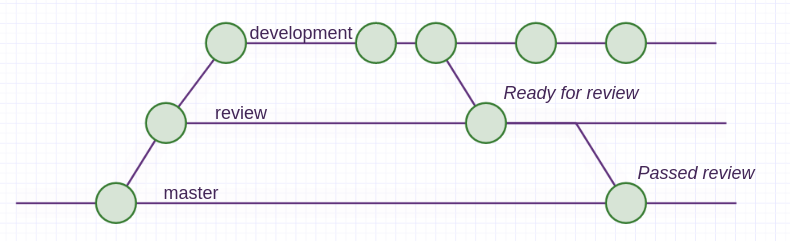
\includegraphics[width=\textwidth]{images/workflow.png}
                \caption{Workflow of the three branches.}
                \label{workflow}
            \end{figure}
        
    \subsection{Change Management \label{versioncontrol}} %10.2
        \subsubsection{E-PUSS}
             E-PUSS is an electronic reporting tool which is used to track and handle
             change management in the project. Details of the tool can be found in appendix B
             in Project Instruction (see section \ref{refs}).

        \subsubsection{Error Reports}
            When a document that has reached baseline requires a change, an error report
            is created in E-PUSS. Exact details of the error report can be found in
            appendix A, under \textit{Problemrapport} in Project Instruction (see section \ref{refs}).

        \subsubsection{Status Reports}
            Status reports will be created in E-PUSS for every configuration item. All changes made to a configuration will be documented in the status report. The following information will be stored:
            \begin{itemize}
                \item Problem ID
                \item Who is resposible for the change
                \item Deadline for the change
                \item The version number of the document \emph{after} the change
                \item Comment
            \end{itemize}
            \noindent *\emph{Optional. Used to match changes with error reports. }

        \subsection{Making Changes To Baseline Documents}
        Before a configuration item has reached baseline, changes to the item
        may occur freely, without any restrictions.
        However, once a configuration item has reached baseline, there are several steps
        that must be taken in order to make changes to it.
        These steps consist of the following:
        \begin{enumerate}
            \item Create an error report.
            \item ECG evalutes the report and decides if it warrants a fix.
                \begin{enumerate}
                    \item If the error is deemed legitimate, ECG proposes a solution and decides who shall be responsible to fix the problem. Once the error is corrected, ECG signs it and the version number is incremented.
                    \item If the error is found to illegitimate, e.g it occured during an outdated test, the report is discarded.
                \end{enumerate}
        \end{enumerate}
        The exact details of this procedure can be found in the Project Instruction (see section \ref{PH}).


    \subsection{Version Naming \& Update}
        The version number is in the format of $X.Y$ where $X$ refers to the baseline
        of the item (in this project, $X$ will be either $0$ or $1$). $Y$ refers
        to which version at the given baseline.
        \\ \\
        How the version number is decided depends on if the item has reached baseline or not.
        \begin{table}[h]
            \centering
            \begin{tabular}{|c|l|}
                \hline
                    \textbf{Baseline} & \textbf{How $Y$ is decided.} \\
                \hline
                    Before & \parbox{.8\textwidth} { \vspace{.2cm}
                            Once a item has been created, the $Y$
                            starts at 1, which results in version $0.1$. When the item is ready for informal
                            review, the $Y$ is incremented to 2. Then, the $Y$ is incremented once for every change to the item until it passes a formal review. This means that before reaching baseline, a item will have a version of at least $0.2$.
                            \vspace{.2cm} } \\
                \hline
                    After & \parbox{.8\textwidth} { \vspace{.2cm}
                        If and only if the procedure described in \ref{versioncontrol}, when a document has reached baseline, results in a modification of the
                        configuration item, the $Y$ is incremented. This means that
                        it is significantly harder to modify a configration item once
                        is has reached baseline. This should make sense since items
                        that have reached baseline have passed formal reviews, which means
                        that they can be seen as valid and reliable.
                        \vspace{.2cm}} \\
                \hline
            \end{tabular}
            \caption{How the $Y$ in $X.Y$ is decided in the version numbering}
            \label{versionnumber}
        \end{table}

\section{Rules and Guidelines} %Assar
    To ensure clear communcation and efficiency PG has set up a series of rules and guidelines. If these rules are not followed, there will be a meeting with the involved parties to determine cause and future actions. 
    
    \begin{itemize}
        \item \textbf{React to information}: Discord has a feature that allows users to react to messages with an emoji. This is a good way to let the sender know that their message has been acknowledged.
        \item \textbf{Mandatory attendance for group meetings and work sessions}: If a group member is unable to attend a meeting they are expected to contact PG and get the information shared during the meeting another way.
        \item \textbf{Weekly time report in E-PUSS every Sunday 17:00}
        \item \textbf{Official project language is English}: Due to english being the dominant language in software development PG has chosen that the project be done in english. This avoids ambigous translations or mixing of languages.
        \item \textbf{Be on time}
    \end{itemize}

\section{Risk Analysis}
    Below are two tables describing the risks, their probability and impact as well as warning signs and solutions
    
    \begin{table}[h]
        \centering
        \begin{tabular}{|l|l|l|}
             \hline
             \textbf{Risk} 
             & \textbf{Probability}
             & \textbf{Impact} \\
             \hline
             Poor Communication 
             & High
             & High \\
             \hline
             Poor work distribution
             & High
             & Medium \\
             \hline
             Problems with the document library
             & Medium
             & Medium \\
             \hline
             Conflicts within the group
             & Low
             & Medium \\
             \hline
        \end{tabular}
        \caption{Risks and impacts}
        \label{tab:my_label}
    \end{table}

    
    \begin{table}[h]
        \centering
        \begin{tabular}{| p{.2\textwidth} | p{.4\textwidth} | p{.4\textwidth} |}
            \hline 
                \textbf{Risk} & \textbf{Warning sign} & \textbf{Solution} \\
            \hline
                Communicationa issues
                & 
                \begin{minipage}[t]{0.4\textwidth}
                    \begin{itemize}
                        \item Information loss.
                        \item People missing meetings.
                        \item Confusion around deadlines. 
                        \item Multiple people working on the same thing.
                     \end{itemize}
                 \end{minipage}
                & 
                \begin{minipage}[t]{0.4\textwidth}
                    \begin{itemize}
                        \item Be very clear \emph{where} we communicate, ask questions.
                        \item Everyone will pay extra attention to all communication channels
                            in use.
                        \item Ensure that the other party of the communcation has recieved
                            and understood the information.
                        \item Practice active listening, ask for confirmation. \\
                     \end{itemize}
                 \end{minipage} \\
            \hline
                Poor work distribution
                &
                \begin{minipage}[t]{0.4\textwidth}
                \begin{itemize}
                    \item Some members experience stress whilst others think the workload is light.
                    \item Missed deadlines.
                    \item Varying quality of work. 
                 \end{itemize}
                 \end{minipage}
                & 
                \begin{minipage}[t]{0.4\textwidth}
                \begin{itemize}
                    \item Take resposibility for your own work.
                    \item Communicate with your group leader.
                    \item If you finish early, ask if anybody needs help. 
                    \item Ask for help if you are falling behind. \\
                 \end{itemize}
                 \end{minipage} \\
            \hline
            Poor planning
            &
                \begin{minipage}[t]{0.4\textwidth}
                \begin{itemize}
                    \item Low attendance at meetings.
                    \item Work is completed long before or after dead lines.  \\
                 \end{itemize}
                 \end{minipage}
            & 
                \begin{minipage}[t]{0.4\textwidth}
                \begin{itemize}
                    \item Plan around deadlines
                    \item Consider individual schedules
                 \end{itemize}
                 \end{minipage} \\
            \hline
            Problems with the document library
            & 
            \begin{minipage}[t]{0.4\textwidth}
                \begin{itemize}
                    \item Work being done twice due to un-updated documents. 
                    \item Reocurring questions about how it works. \\
                 \end{itemize}
                 \end{minipage}
            & \begin{minipage}[t]{0.4\textwidth}
                \begin{itemize}
                    \item Hold lectures breaking down the steps
                    \item Use cheat sheats and provide additional resources
                 \end{itemize}
                 \end{minipage} \\
            \hline
            Conflicts within the group
            & 
                \begin{minipage}[t]{0.4\textwidth}
                \begin{itemize}
                    \item Tension during meetings. 
                    \item Group members are silent during meetings due to fear of judgement.
                 \end{itemize}
                 \end{minipage}
            & \begin{minipage}[t]{0.4\textwidth}
                \begin{itemize}
                    \item Put your pride aside and focus on a solution.
                    \item Have an understanding for others.
                    \item Tell a leader if you feel like you are being treated unfairly.
                    \item Ask somebody to mediate in a conflict \\
                 \end{itemize}
                 \end{minipage} \\
            \hline
        \end{tabular}
        \caption{Warning signs and solutions}
    \end{table}
    
\end{document}